\chapter{STUDYING POLICY ATTACKS TRANSFERABILITY}
\label{sec:exp1}

This section reports the results of the first of the three experiments included in this thesis. It evaluates different policy attacks focusing on their transferability and drawing some insights about their performance under different scenarios.

\section{Studying policy attacks transferability}
The first experiment included in this work consists of studying the transferability over different policies and algorithms of some policy attacks so as to have an idea of their robustness and gain a better understanding of the effectiveness and proprieties of the employed attacks. In particular, we are interested in understanding how vulnerable neural network policies are against adversarial policies and how their effectiveness is affected by the way those policies are trained and the amount of knowledge is available to the attacker with respect to the target policies. Their robustness is measured by plotting the {\it reward vs attack frequency curves} of different policy attacks under a fixed threat model for each curve with the aim to measure the reduction of the agent's reward as the attack frequency increases. The experiments have been conducted on three popular reinforcement learning algorithms: DQN, A2C, and PPO with policies trained on an environment belonging to the Atari games category, namely Pong. Besides, the five policy attack methods that have been compared include:
\begin{itemize}
    \item Uniform attack;
    \item Strategically-timed attack;
    \item Critical point attack;
    \item Critical strategy attack;
    \item Adversarial policy.
\end{itemize}

\subsection{Environments}
All the environments where the policies have been trained consist of common Atari games included in the Gym library \cite{brockman2016openai}. Hence, the observations are RGB images of the screen, which are arrays of shape (210, 160, 3). Moreover, each action is repeatedly performed for a duration of \(k\) frames, where \(k\) is uniformly sampled from \([2, 3, 4]\). To represent temporal information, 4 observations are stacked together, converted to grey-scale, and scaled down to have a shape of (84, 84, 1) pixels.
\subsubsection{Pong}
In this environment, both the agent and the opponent control a paddle which can be only moved vertically across the screen to hit a ball back and forth. Each player scores one point when the other player fails to return the ball to the other and their goal is to reach eleven points before the opponent. The player on the right is controlled by the agent and the one on the left is controlled by a simple hard-coded AI.

\subsection{Experiments settings}
\subsubsection{Algorithms hyper-parameters}
To implement and train the reinforcement learning policies with their corresponding algorithms, it has been used the framework Tianshou \cite{tianshou} based on Pytorch. Starting to describe algorithms specifications, the DQN variant adopted in this work takes advantage of a prioritized experience replay \cite{schaul2016prioritized} of size 100k to sample more frequently the most critical observations, that is those observations where the discrepancy between the Q-values of the online and target network is more significant, so to lead to faster training. It has also been implemented Double Q-network to decouple the selection of the action from the evaluation and reduce overestimation, and multi-step learning with an estimation of 3 steps so to take advantage of the bootstrapped sequences of transitions to improve the target value accuracy. Training has been conducted for a total of 10M frames with \(\epsilon\) linearly decaying from 1 to 0.05 during the first 1M frames to encourage exploration. The target network has been updated with the weights of the online network every 5000 frames. Regarding A2C and PPO algorithms, the policy has been trained for 10M frames and updated with trajectories of 128 steps and a batch size of 32. The advantage has been computed using GAE with \(lambda\) equal to 0.95. The value loss and the entropy loss have been given a weight of 0.5 and 0.01 respectively. For PPO the clipping ratio is 0.2. Other common parameters used in all the three algorithms are a learning rate of 0.0001 and \(gamma\) of 0.99 used to define the importance of long-term rewards. To speed up training, all policies have been trained on 16 parallel environments. In order to measure attack policy transferability, for each environment have been trained two policies using different seeds but with their performance remaining similar. The average reward of the surrogate policy of each environment doesn't differ more than 10\% of the mean reward of the corresponding primary policy. Table \ref{table:2} reports the average score over 100 episodes for the three different algorithms.

\begin{table}
  \centering
  \caption{Average score over 100 episodes for policies trained with DQN, A2C, and PPO. It can be clearly seen that PPO, being a more sophisticated algorithm than the other two also performs much better. Pong is easy enough that most algorithms can successfully train a policy to defeat the opponent.}
  \begin{tabular}{cccc}
    \toprule
    Environment & DQN & A2C & PPO \\
    \midrule
    Pong & 20 & 20 & 21 \\ 
    \bottomrule
  \end{tabular}
  \label{table:2}
\end{table}

\subsubsection{Image adversarial attacks settings}
All the evaluated policy attacks exploit FGSM to craft perturbations to generate adversarial observations. The reasons we have chosen to adopt a simple method like FGSM over more sophisticated white-box attacks are the following: first of all, FGSM is a one-shot method that can craft adversarial perturbation in just one iteration, thus it is many times faster than iterative ones such as PGD. Given the number of times the attack is required to be executed to hamper thousands of policy trajectories, evaluating an iterative method could be not worth the time in correspondence of a moderate gain in attacks success rate. Secondly, the experiments presented in section \ref{sec:exp3} empirically show that, when attacking Atari observations, FGSM doesn't perform worse than iterative methods under the same distance norm and perturbation strength. All perturbations have been computed under \(l_\infty\) norm with a distance of \(\epsilon=0.05\).

\subsubsection{Policy adversarial attacks settings}
Next, it is explained how attack-frequencies relative to the evaluated policy attacks have been defined in order to generate the corresponding curves. Among the included attacks, the simplest method is the uniform attack where it can be directly tuned a predefined frequency hyper-parameter, thus changing the probability to attack each observation. Strategically-timed attack and adversarial policy exploit the parameter \(beta\) to fine-tune their frequency. Higher values of \(beta\) mean that the difference between the most and the least likely actions should be higher in order to attack the corresponding observation, thus meaning it has been encountered a more critical state. When \(beta=0\) it results that every frame is attacked and a value of \(beta\) close to 1 corresponds to very sparse but effective attacks. Under this criteria, critical states correspond to those states where choosing a particular action has a significant influence on the reward over the future states. Since the original method doesn't provide a way to define a certain attack frequency, the hyper-parameter \(beta\) has also been added to adversarial policy attack so to tune its attack rate. Finally, the attack frequency of the critical point and critical strategy attack is determined by the two parameters \(n\) and \(m\) which affect the length of the adversarial strategies. When \(n=m\), both methods perform attacks over all frames and their frequency reduces as the difference \(m-n\) grows.

Besides critical point attack, all the other policy attacks can be generally used to attack different environments just by fine-tuning their hyper-parameters without requiring any extra configuration. However, critical point attack is based on a divergence function \(T\) to estimate how critical is any observation. In this context, critical observations are those observations where the likelihood to fail the episode is higher. Adapting this concept to the evaluated environments, the divergence function is correlated to the probability that the ball would pass over the paddle, giving one point to the opponent in the case of Pong. This probability is estimated as the distance between the center of the paddle and the ball along the \(y\)-axis for Pong. The concept behind this function is that the further the distance between the ball and the paddle along the corresponding axis, the more difficult is for the normal policy to catch the ball. A more sophisticated divergence function would have been designed by taking into consideration also the direction of the ball. Unfortunately, it would have been more complex to implement since it would involve a sequence of stacked frames and precise algorithms to estimate the direction of the ball by comparing its shape and position over different frames. In practice, a model could take as input sequences of stacked observations but in this work we consider only the last one to compute the value of the divergence function. Moreover, designing an optimal divergence function is out of the scope of this thesis project. An example of the behavior of the divergence function for the game of Pong is showed in figure \ref{figure:t-func}.

\begin{figure}
  \centering
  \subcaptionbox{Safe state \label{fig:subfig-a}}
    {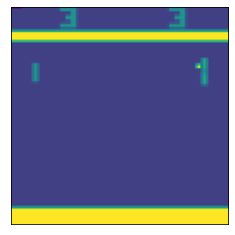
\includegraphics[width=0.32\linewidth]{images/Pong-Tfunc-good.png}}
  \subcaptionbox{Uncertain state\label{fig:subfig-b}}
    {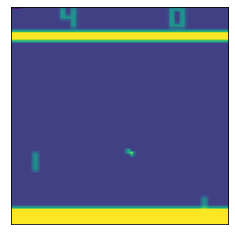
\includegraphics[width=0.32\linewidth]{images/Pong-Tfunc-normal.png}}
    \subcaptionbox{Dangerous state\label{fig:subfig-c}}
    {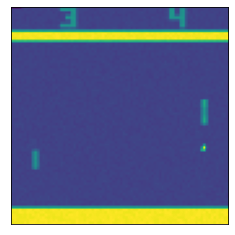
\includegraphics[width=0.32\linewidth]{images/Pong-Tfunc-bad.png}}
  \caption{Example of the behavior of the divergence function \(T\) for the game of Pong: the observation on the left (a) has a very low level of \(T\) since the probability that the agent fails is 0. The observation in the middle (b) presents a discrete \(T\) since considering the ball moving simply toward the right of the screen along the \(x\)-axis the agent can still make the ball bounce back. The third observation (c) has a very high value of \(T\) since there is no way the agent can save the ball.}
  \label{figure:t-func}
\end{figure}

\section{Results}
The next three sections show the {\it reward vs attack frequency curves} of all the evaluated policy attacks under a fixed threat model so to measure their effectiveness and their transferability against policies and algorithms. When analyzing the obtained results, sometimes we may refer to the curve of the policy attacked without transferability as baseline policy. In addition, we may sometimes intend as {\it attacking with a surrogate policy} or {\it attacking with a surrogate algorithm} as crafting adversarial perturbations exploiting a surrogate policy/algorithm to attack the target policy. Let's also remind that the purpose of these experiments is not only to evaluate the efficacy of different attack methods but to study their transferability proprieties. Hence, the relative value of each curve with respect to the other ones is more important than their individual absolute value.

\subsection{Attacking Pong-DQN}
The curves relative to this experiment are depicted in figure \ref{figure:pong-dqn}. We observe that in the case of uniform attack, the average rewards decrease from 20 to -20 almost linearly as the attack frequency increases from 0 to 0.5. For higher frequencies we didn't observe a larger drop in reward, thus meaning that the victim policy already performs close to the worst possible case. On the evaluated environment, uniform attack also shows good transferability both in terms of policy and algorithm. In particular, crafting adversarial observations with a similar policy yields similar results to attacking the baseline policy, obtaining almost identical performance for lower attack frequencies. Perturbations crafted on the other two algorithms, namely A2C and PPO, still successfully fool the victim agent with their curves following the trend of the baseline but maintaining an average reward difference of about 5 points.

Analyzing the curves relative to the strategically-timed attack, we can observe that the attack frequency is several grades of magnitude lower than uniform attack and is the lowest among all the examined policy attacks. In the frequency interval taken into consideration, which varies from 0.002 to 0.012, the corresponding average reward drops from a little more than 10 to less than -15 for the baseline policy which follows an almost linear decay. However, considering that this time adversarial observations are crafted in a targeted way, transferability seems to be less effective than it was for uniform attack. While attacking with policy transferability still yields results relatively closer to the baseline, perturbations crafted on the two on-policy algorithms often fail to fool the agent, thus requiring more attacks to provide meaningful results. 

Critical point attack has attack frequencies varying from 0.01 to 0.09, interval in which the reward falls from 20 to -15. As opposed to the previous two attacks, perturbations crafted under the surrogate policy don't work much better than the perturbations crafted on the policy trained with the other two on-policy attacks. Nevertheless, DQN policy transferability still seems to work a little better than A2C and PPO algorithm transferability as the attack frequency increases.
The curves of critical point and critical strategy attack are very similar both in terms of rewards and frequencies. However, both methods can't reduce the agent's reward to less than -15 in the given frequency interval. 

Finally, adversarial policy attack seems to perform the worst. The curves representing the two algorithms' transferability are very far from the other two curves and struggle to lower the reward to less than 10 points. The curve corresponding to policy transferability is also much weaker than the baseline but they follow the same trend and it is able to lower the average reward to less than 0 points. Overall, we can conclude saying that DQN is not a very robust algorithm since perturbations crafted with surrogate policies still fool the victim model with performance similar to directly attacking the victim policy. In fact, the closer are the curves to the baseline, the less robust is the target algorithm.

\begin{figure}
  \centering
  \subcaptionbox{Uniform attack \label{fig:subfig-a}}
    {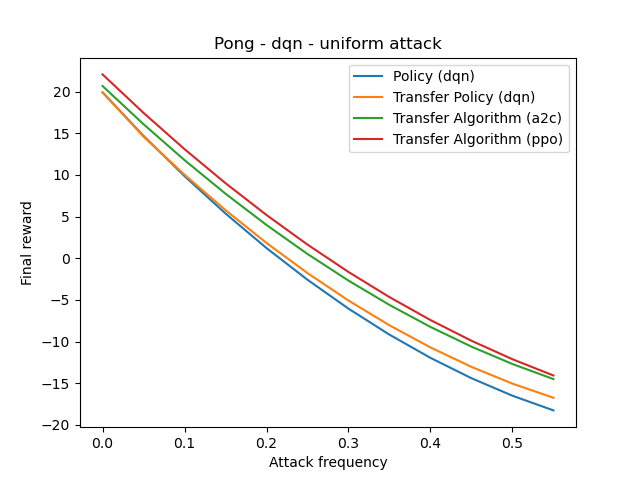
\includegraphics[width=0.49\linewidth]{images/exp1/dqn-pong-uniform.png}}
  \subcaptionbox{Strategically-timed attack\label{fig:subfig-b}}
    {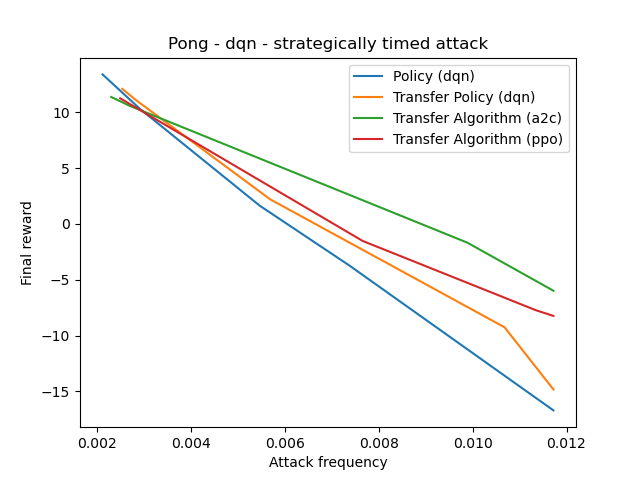
\includegraphics[width=0.49\linewidth]{images/exp1/dqn-pong-strategically_timed.png}}
  \subcaptionbox{Critical point attack\label{fig:subfig-c}}
    {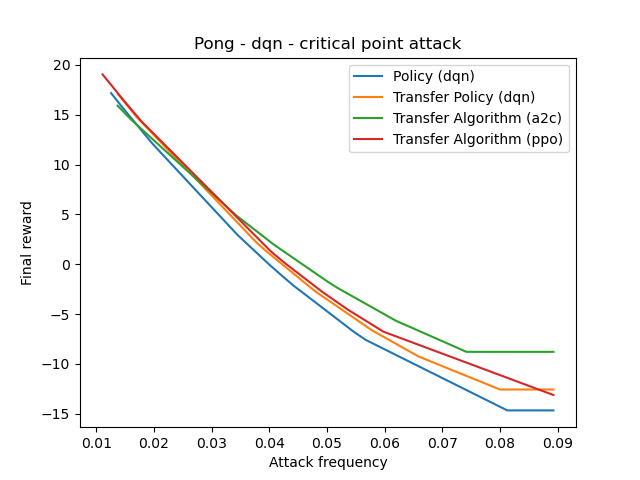
\includegraphics[width=0.49\linewidth]{images/exp1/dqn-pong-critical_point.png}}
  \subcaptionbox{Critical strategy attack\label{fig:subfig-d}}
    {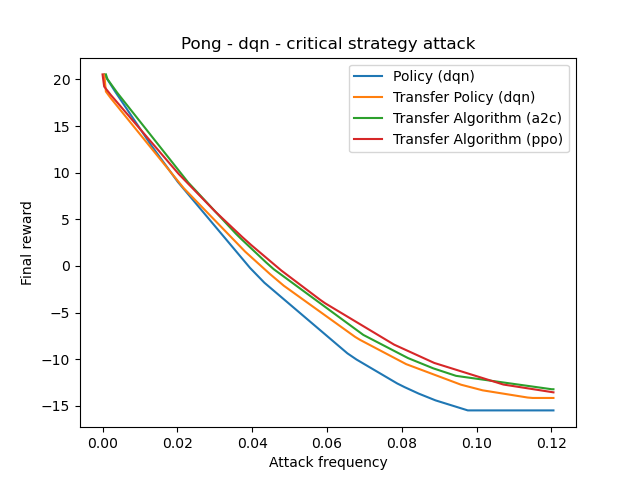
\includegraphics[width=0.49\linewidth]{images/exp1/dqn-pong-critical_strategy.png}}
  \subcaptionbox{Adversarial policy attack\label{fig:subfig-e}}
    {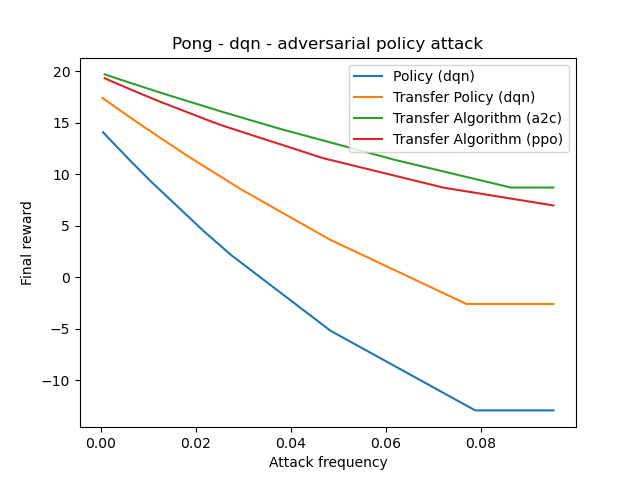
\includegraphics[width=0.49\linewidth]{images/exp1/dqn-pong-adversarial_policy.png}}
  \caption{The {\it reward vs. attack frequency} curves of 5 policy attacks with FGSM under the \(l_\infty\) norm attacking a Pong-DQN policy.}
  \label{figure:pong-dqn}
\end{figure}

\subsection{Attacking Pong-A2C}
The curves relative to the A2C policy are shown in figure \ref{figure:pong-a2c}. Beginning analyzing uniform attack, we can see that the curve of the baseline is similar to its corresponding DQN version but the performance of the surrogate policies drop considerably. Attacks with the surrogate similar policy still follow the trend of the baseline with a rapid decrease of the agent's reward for frequencies increasing from 0 to 0.25 and a more amortized decline until a frequency of 0.5. Attacks exploiting a surrogate algorithm never inflict too much damage in the considered interval with PPO producing the least effective perturbations. Adversarial observations crafted with DQN struggle to lower the average reward of the target policy to below 0 in the given frequency interval while PPO slowly reduces the rewards from 20 to 10. Strategically-timed attack once again benefits of a very low attack frequency. However, the robustness of A2C deeply impacts the effectiveness of the attacks with the surrogate policies. The baseline reduces the rewards from 20 to -15 attacking less than 2\% of the observed frames. Same as in uniform attack, adversarial examples generated attacking PPO need a higher attack rate to reduce the rewards by 10 points and DQN performs even worse. Also the baselines of the curves of critical point and critical strategy attack are similar to the baseline of their corresponding curves obtained in the previous section when attacking the DQN agent. As it was for the other methods, the surrogate policies perform much worse, with the attacks based on algorithm transferability suffering the most. Also in the case of adversarial policy, the adversary doesn't perform very well and its baseline resembles the one of uniform attack. In fact, it needs to increase the attack frequency to over 0.3 to achieve successful results. Attacks with DQN and PPO present very similar curves, both decreasing steadily to reduce the average reward to -5. We can then draw out the conclusion that A2C algorithm is more robust than DQN, in particular, it seems to resist very well against attacks with surrogate policies trained with different algorithms. In fact, all attacks show poor algorithm transferability and discrete policy transferability.

\begin{figure}


  \centering
  \subcaptionbox{Uniform attack\label{fig:subfig-a}}
    {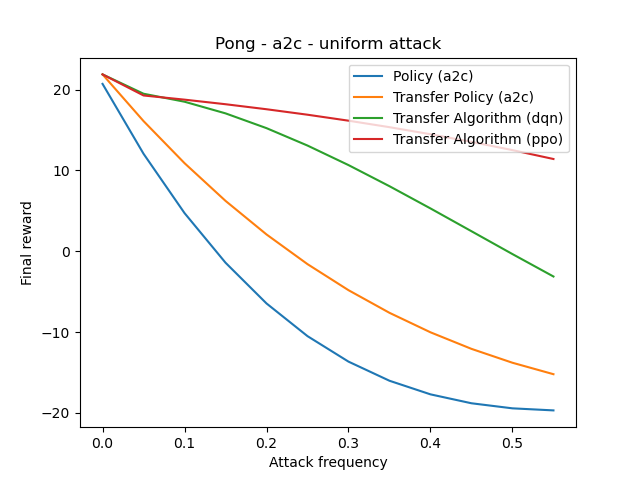
\includegraphics[width=0.49\linewidth]{images/exp1/a2c-pong-uniform.png}}
  \subcaptionbox{Strategically-timed attack \label{fig:subfig-b}}
    {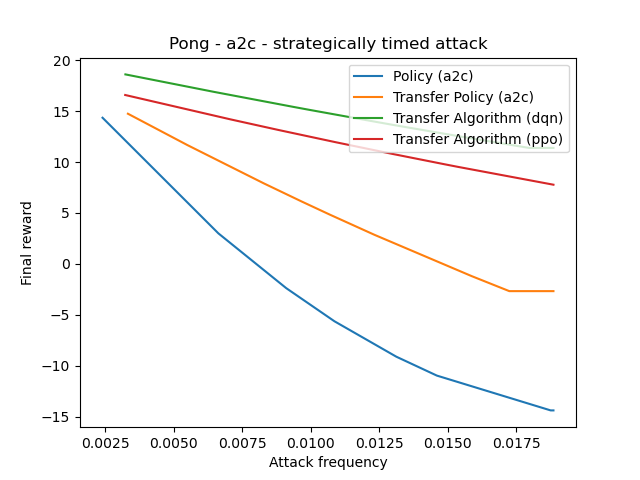
\includegraphics[width=0.49\linewidth]{images/exp1/a2c-pong-strategically_timed.png}}
  \subcaptionbox{Critical point attack\label{fig:subfig-c}}
    {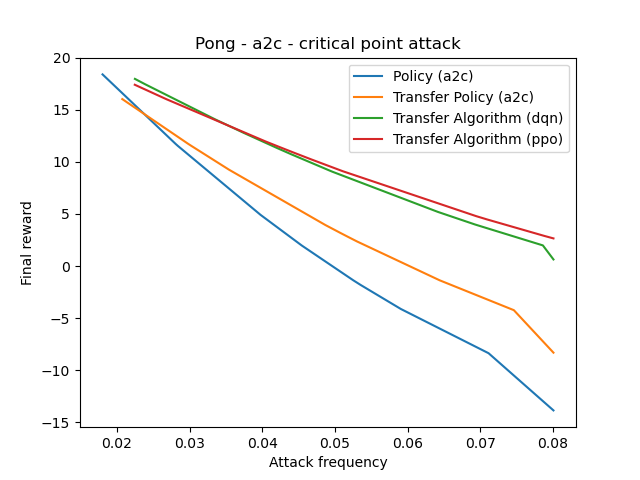
\includegraphics[width=0.49\linewidth]{images/exp1/a2c-pong-critical_point.png}}
  \subcaptionbox{Critical strategy attack\label{fig:subfig-d}}
    {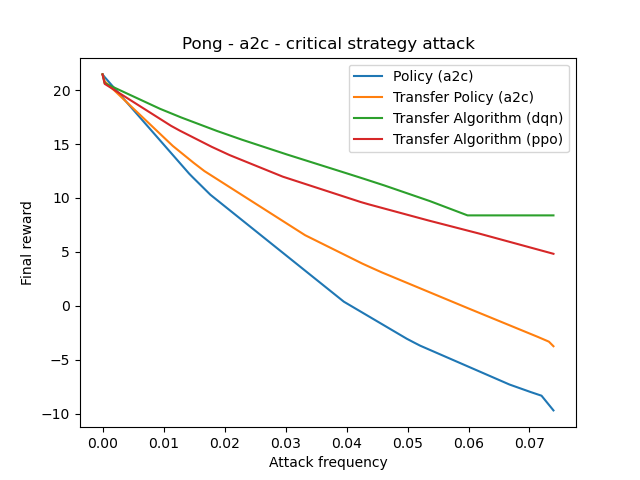
\includegraphics[width=0.49\linewidth]{images/exp1/a2c-pong-critical_strategy.png}}
  \subcaptionbox{Adversarial policy attack\label{fig:subfig-e}}
    {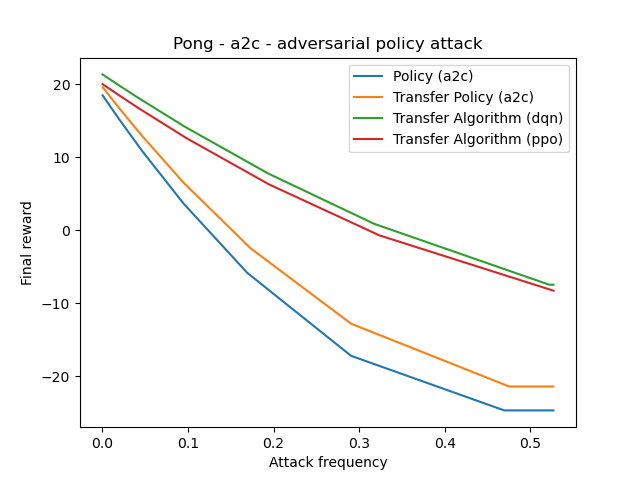
\includegraphics[width=0.49\linewidth]{images/exp1/a2c-pong-adversarial_policy.png}}
  \caption{The {\it reward vs. attack frequency} curves of 5 policy attacks with FGSM under the \(l_\infty\) norm attacking a Pong-A2C policy.}
  \label{figure:pong-a2c}
\end{figure}

\subsection{Attacking Pong-PPO}
The last set of charts depict the curves relative to the policy trained with PPO and it is shown in figure \ref{figure:pong-ppo}. Starting from the uniform attack, nothing new appears here with respect to the charts of the uniform attack relative to the other two algorithms. All curves follow the trend of the baseline but the adversarial examples generated with transferability are this time less effective. Attacks crafted with DQN are the ones performing the worst. Strategically-timed attack seems not to be able to attack as easily as it did against DQN. In fact, it requires a relatively higher attack frequency to achieve similar performance. Moreover, same as in the case of A2C, attacks with surrogate models trained with different algorithms, have to put more effort to decrease the average reward of the victim agent. Conversely, policy transferability still works discretely well. Critical point and critical strategy attack demonstrate good transferability and similar results, thus meaning that in the environment of Pong a hand-crafted divergence function is unnecessary to elaborate good attack strategies. Surprisingly, adversarial policy attack seems to work better than it did when attacking A2C. It can almost linearly lower the agent's average reward from 20 to 0 attacking no more than 20\% of the frames. and it also owns a better transferability property than it had against A2C and DQN. Overall, PPO seems to be a little more robust than DQN but less robust than A2C. In terms of transferability all attacks, except for strategically-timed attack, are able to craft effective adversarial observations using their respective surrogate policies. Strategically-timed attack still works very well under policy transferability but fails when attacking with different algorithms.

\begin{figure}
  \centering
  \subcaptionbox{Uniform attack \label{fig:subfig-a}}
    {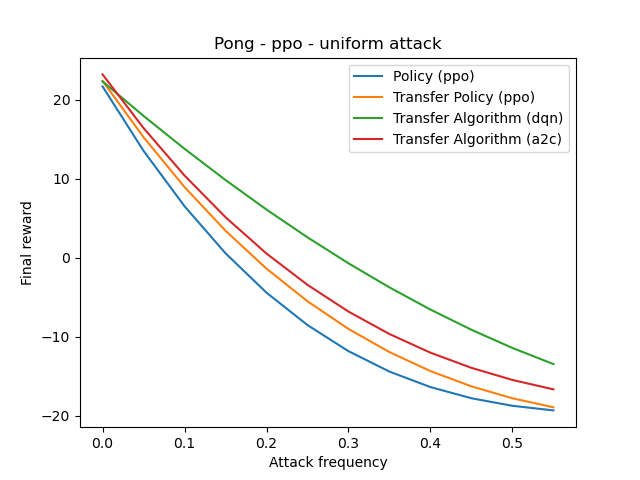
\includegraphics[width=0.49\linewidth]{images/exp1/ppo-pong-uniform.png}}
  \subcaptionbox{Strategically-timed attack\label{fig:subfig-b}}
    {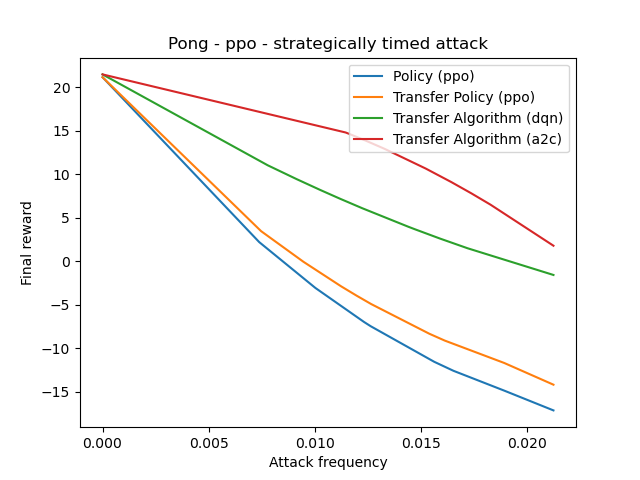
\includegraphics[width=0.49\linewidth]{images/exp1/ppo-pong-strategically_timed.png}}
  \subcaptionbox{Critical point attack\label{fig:subfig-c}}
    {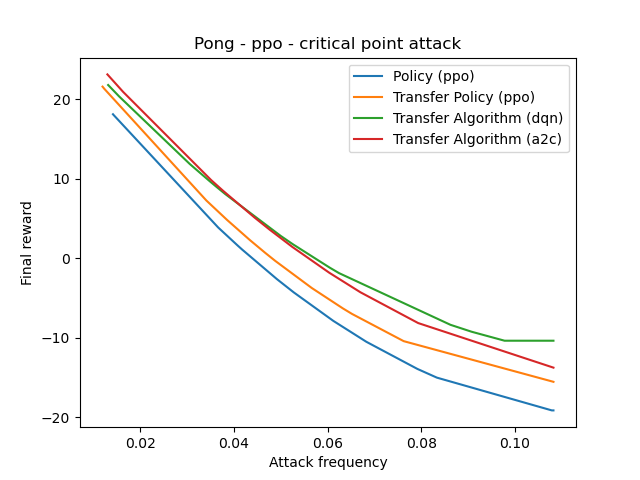
\includegraphics[width=0.49\linewidth]{images/exp1/ppo-pong-critical_point.png}}
  \subcaptionbox{Critical strategy attack \label{fig:subfig-d}}
    {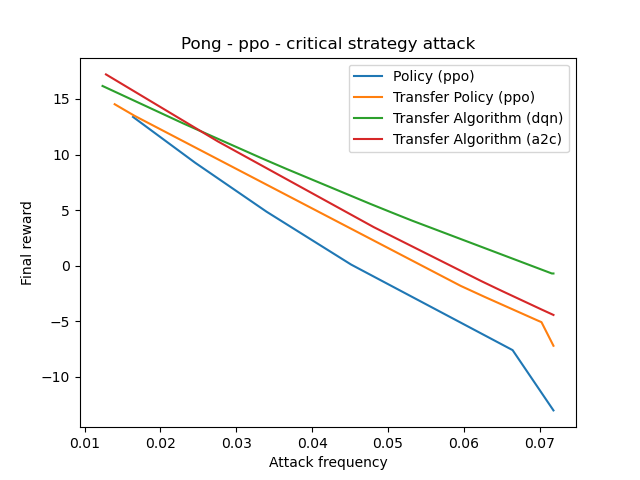
\includegraphics[width=0.49\linewidth]{images/exp1/ppo-pong-critical_strategy.png}}
  \subcaptionbox{Adversarial policy attack \label{fig:subfig-e}}
    {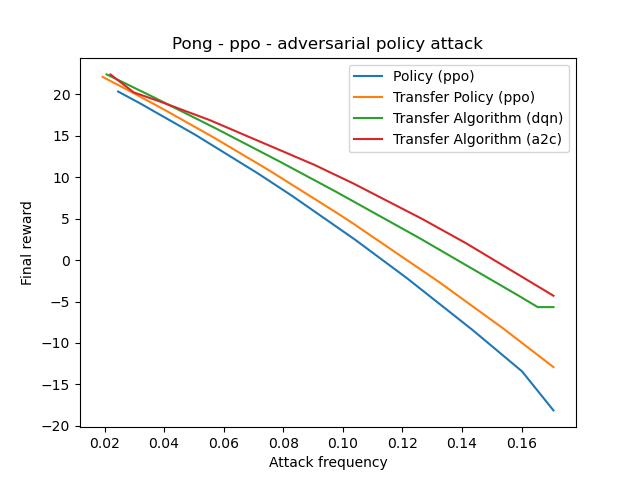
\includegraphics[width=0.49\linewidth]{images/exp1/ppo-pong-adversarial_policy.png}}
  \caption{The {\it reward vs. attack frequency} curves of 5 policy attacks with FGSM under the \(l_\infty\) norm attacking a Pong-PPO policy.}
  \label{figure:pong-ppo}
\end{figure}

\section{Findings}
This section analyses the policy attack methods that have been evaluated in this experiment and draws some conclusions about their usage, effectiveness, and drawbacks. It also points out some future research directions to improve those attacks and makes insightful comparisons among similar methods.

\subsection{Uniform attack vs strategically-timed attack}
Not surprisingly, uniform attack is the most simple but also the weakest attack that has been examined in the present evaluation. However, it is very fast and is compatible with untargeted image attacks, thus allowing the exploration of other image attacks such as Deepfool that only work under untargeted settings \cite{moosavidezfooli2016deepfool}. Interestingly, strategically-timed attack achieves the best performance under the lowest frequencies. The reason behind its excellent performance is that this method has specifically been designed to work under low attack frequencies attacking only in correspondence with the most critical observations. Being its attacks very sparse, it takes more frames to make the victim agent fail. Hence, resulting in a very low attack frequency. The intelligent way strategically-timed attack decides whether to attack an observation or not could be also borrowed to other methods such as uniform attack to lower their frequency while limiting the drop in performance. In this work, this technique has been applied also to the adversarial policy attack to vary its frequency. One possible drawback of this technique is that it may miss some observations that apparently don't seem critical but that attacking them may lead to worse states in the future steps, a drawback that has more important consequences in the case of the adversarial policy attack.

\subsection{Critical point vs critical strategy attack}
Critical point attack and critical strategy attack are constrained by the hyper-parameter \(n\) which, forcing the two methods to attack every observation over sequences of \(n\) frames, might result in some unnecessary attacks. Overall, the attack frequency is largely influenced by the \(m\) parameter which defines the number of steps taken without attacking the policy of the agent. Higher values of \(m\) comport a decrease of the attack frequency but also lead to a potential risk of missing some critical states which it would have been worth attacking. In fact, the last \(m-n\) observations of an observed trajectory are completely ignored by both attacks. Different frequencies are thus generated varying \(n\) and \(m\). Going more deeply into understanding their behaviors, critical point attack relies on a divergence function to estimate how critical is the last state of a trajectory defined by a strategy. However, both the strategy that defines some sequences of malicious actions and the divergence function of critical point attack are hand-crafted, which means that they require some domain knowledge to be designed by a human. While a strategy that works for a certain environment may still work quite well in similar environments, a specific divergence function will not work in other environments, even for similar ones. For instance, a strategy that only repeats the same action is considered a malicious strategy for almost all the Atari environments, but clearly, this transferability property may not be true for some other environments. In contrast, critical strategy attack depends on the cumulative reward over a trajectory to determine the maliciousness of a strategy: the lower the reward the more malicious a strategy is. However, what makes reinforcement learning challenging is exactly the sparsity of the rewards. This means that the value of most trajectories will be zero. On one hand, this is a positive property since adversarial strategies will always aim to prevent the agent to increase its score, eventually leading it to fail the episode or lose one life. On the other hand, with many strategies preventing the agent to get any reward along, it's not easy to determine which one may continue to lead the agent to more malicious states in the future steps. For both attacks, the special case where \(m=n\) means attacking every frame and both attacks are more effective as \(n\) increases and the difference \(|m-n|\) reduces. Furthermore, the hyper-parameter \(n\) has influence on the number of adversarial strategies to be tested. Supposing \(a\) to be the number of actions of an environment and the strategies to be all possible combinations of \(n\) actions, \(a^n+a*(m-n)\) strategies will be evaluated with \(n\) adding an exponential computational cost since more strategies will be evaluated. Thus, the way to generate adversarial strategies should be carefully crafted. Overall, critical point attack performs slightly better than critical strategy but it depends on a divergent function to be computed on the input observations which sometimes could be a challenging task.

\subsection{Adversarial policy and future search directions}
Given the results presented in this section, apparently adversarial policy attack is the one performing the worst. The reason behind this is that this method doesn't have a real mechanism to control and vary its frequency. Hence, it borrows the technique used by strategically-timed attack. The difference between the two is that while the strategically-timed attack executed the least likely action, adversarial policy attack crafts perturbations such that the victim agent executes a specific action predicted by the network implementing the adversarial policy. In fact, in adversarial policy attack, all actions are equally important since the goal here is to lead the agent toward a certain state where failure is inevitable. However, missing one or a few steps because wrongly considered as not critical may lead to other less malicious policies. Generally, this method as well as critical point and critical strategy, focuses on making the agent fail faster rather than slowly sabotage it as uniform attack and strategically-timed attack do. However, blindly attacking each frame is still not an elegant solution to make these attacks effective. Attacking more observations not only requires more computational power but also increases the possibility of the attacker being detected. If hand-crafting a mechanism to determine when to attack is not enough for such more complex methods, then machine learning is once again the answer. Future research directions might then focus also on {\it when to attack} rather than {\it how to attack}, thus learning to predict critical observations along the corresponding malicious action and even learning to limit the number of attacks so to control the frequency. \cite{sun2020stealthy} pioneers this work with antagonist attack.

\subsection{Attack feasibility in common scenarios}
Another point that is important to mention is that strategically-time attack takes advantage of the logits or probability of the predicted actions in order to attack the victim agent. However, this knowledge is not always available under common threat models. Thus, although the above-mentioned attack seems to work extremely well under experiment settings, in practice it may result ineffective in real-world scenarios. In contrast, to use uniform attack the adversary only needs to know the action predicted by the model representing the policy so to cause it to take another random action. This knowledge is usually more commonly available than the actions probabilities but it is still a limiting constraint to make the attack work. However, this contrast could be relaxed by assuming the target agent to have taken a certain action, even a random action, and consequently use it to craft the corresponding perturbations. Critical point and critical strategy both need a simulator of the environment to assert the value of their strategies. In the best-case scenario, a copy of the state of the environment could be used so as to exactly know the outcome of each strategy. In fact, both methods could take actions in the environment according to the actions defined in a strategy, compute the value of the last observation or the value of the trajectory and then revert it to the saved state so to evaluate the next strategy. If retrieving the state of the environment is not possible, then it should be engineered other ways to make a simulation of the environment that is as close as possible to the original one. The authors of critical point attack proposed to train a neural network that given an observation and an action it predicts the next observation. An interesting solution is the one introduced in \cite{kim2020learning} which trains a variant of GAN to learn a simulator by simply watching an agent interact with the environment. In those circumstances where, for any reason, a simulation of the environment is not available, attack strategies can still be computed based on a simulation of similar environments or simply designing some strategies that intuitively may be malicious for the target environment regardless of its current state. The only requirement adversarial policy attack needs in order to attack its target is to have access to the input observations. Therefore, this method is more flexible since it can work under different threat models. However, it still needs to be trained in the same environment of the victim policy before it can be used to attack it. Let's remind that all the policy attacks evaluated in this thesis work only under the condition that input observations can be modified. Table \ref{table:atk_req} summarizes the requirements of each policy attack to work properly.

\begin{table}
  \centering
  \caption{Requirements needed for each evaluated policy attack method to work properly.}
  \begin{tabular}{ccccc}
    \toprule
    Attack method & Observations & Environment & Pred action & Actions probs              \\
    \midrule
     Uniform Attack & V & - & V & - \\ 
 Strategically-Timed Attack & V & - & - & V \\
 Critical Point Attack & V & V & - & - \\
 Critical Strategy Attack & V & V & - & - \\
 Adversarial Policy & V & Only for training & - & - \\
    \bottomrule
  \end{tabular}
  \label{table:atk_req}
\end{table}

\subsection{Online vs offline attacks}
Uniform attack, strategically-timed attack, and adversarial policy attack are relatively fast attacks. In fact, excluding the time the image attack method takes to generate the adversarial perturbations, the first two methods only involve a few linear computations while the third one requires one forward pass of its network. Hence, those three attacks, combined with a fast image attack method, are suitable to attack in an online way following the stream of states observed by the target agent. Conversely, critical point and critical strategy attack need to explore and assert the damage of different strategies before start attacking and this operation should be repeated every \(n+m\) frames. This bottleneck makes these two attacks too slow to be executed in an online way but more useful to attack offline when time is not a constraint. Nevertheless, in real life scenario is more common to have to attack online rather than offline.